\documentclass[letterpaper,twocolumn,amsmath,amssymb,pre,aps,10pt]{revtex4-1}
\usepackage{graphicx} % Include figure files
\usepackage{color}
\usepackage{nicefrac} % Include for inline fractions

\newcommand{\red}[1]{{\bf \color{red} #1}}
\newcommand{\green}[1]{{\bf \color{green} #1}}
\newcommand{\blue}[1]{{\bf \color{blue} #1}}
\newcommand{\cyan}[1]{{\bf \color{cyan} #1}}

\newcommand{\davidsays}[1]{{\color{red} [\green{David:} \emph{#1}]}}
\newcommand{\jpsays}[1]{{\color{red} [\blue{Jordan:} \emph{#1}]}}
\newcommand{\tssays}[1]{{\color{red} [\cyan{Tanner:} \emph{#1}]}}

\begin{document}
\title{Stochastic Approximation Monte Carlo with Dynamic Update
Factor (SAD)
}

\author{Jordan K. Pommerenck} \author{Tanner T. Simpson}
\author{Michael A. Perlin} \author{David Roundy}
\affiliation{Department of Physics, Oregon State University,
  Corvallis, OR 97331}

\begin{abstract}
  We present several histogram methods and compare the performance and
  efficiency at treating the square-well fluid.
\end{abstract}

\maketitle

\begin{figure}
  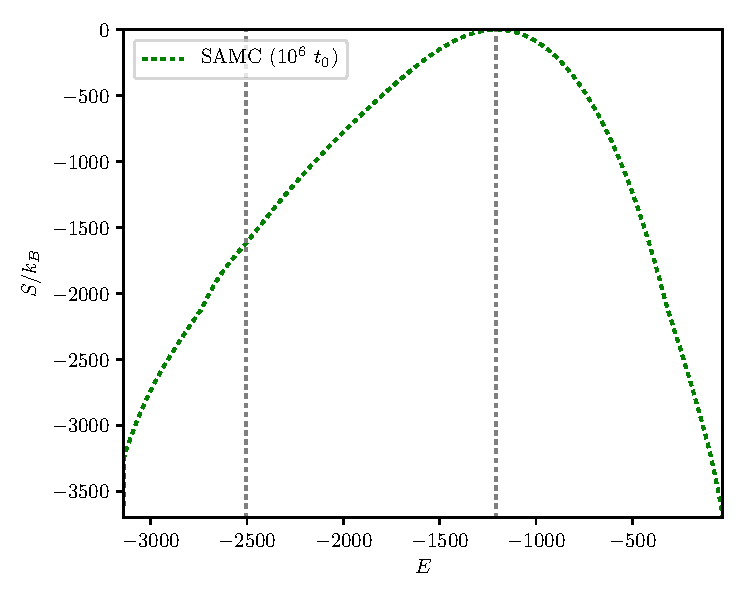
\includegraphics[width=\columnwidth]{figs/N500-lndos-comparison}
  \caption{Put this in the right place}
\end{figure}

\section{Introduction}
Over the past several decades a number of flat histogram Monte-Carlo
simulation algorithms have been developed which calculate the
thermodynamic properties of various systems for all temperatures.  The
development began with the original histogram method, which used a
single canonical Monte Carlo simulation to predict properties for
nearby temperatures~\cite{ferrenberg1988new}.  For large simulations
this approach is limited to a narrow temperature range because a single
canonical simulation explores only a small range of energies.  This led
to a variety of ``broad'' (or ``flat'') histogram
methods~\cite{penna1996broad, penna1998broad, swendsen1999transition,
wang2001determining, wang2001efficient, trebst2004optimizing}, which
attempt to explore a wide range of energies.  These methods also
benefit in that they are unlikely to be trapped in a low enetropy state.

Wang and Landau introduced an algorithm that uses an update factor and
a statistical histogram to compute the density of states of a given
system~\cite{wang2001determining, wang2001efficient}.  While the method
is incredibly powerful, it has several user-defined parameters.  This
can make its application to a variety of systems something of an
art-form since the user needs to determine the ideal parameters for the
particular system being studied.  Also, detailed balance is violated
(although only for short periods of time), ensuring that convergence is
not guaranteed.  This raises several questions such as when the method
does converge, what rate will the method converge to the correct
density of states. Also, how can the user appropriately decide what
parameters to choose so that the algorithm solves the problem in the
most ideal way.

Transition Matrix Monte Carlo~\cite{wang1999transition,
swendsen1999transition, fitzgerald2000monte} became an attractive
complimentary simulation algorithm to Wang-Landau, in that, if detailed
balance is ensured, the system is guaranteed to converge.  Unfortunately,
the algorithm can be considerably more difficult to implement when
compared to Wang-Landau: in particular, due to the infinite temperature
transition matrix~\cite{wang2002transition}.  Also, the time necessary
for the density of states to converge could be considerable
due to the algorithm spending too much time exploring low energy states.
Unlike WL, TMMC does not require a prior knowledge of the energy range of
the system.

Shell et al.~\cite{shell2003improved, shell2004flat} originially
implemented Wang-Landau Transition Matrix Monte Carlo (WL-TMMC) in an
effort to quickly explore the energies of a given system using WL then
switch over to TMMC to guarantee convergence. Considerable effort has
been spent trying to determine the flatness criteria and cutoff for the
WL portion, but there remains no rigorous systematic way to determine
these parameters~\cite{rane2013monte}.  The algorithm is first run for
several trial simulations and/or `experience' is used to determine the
best parameters for a users particular system of
study~\cite{siderius2013use}.

Around the same time, the convergence rate for WL was being
explored~\cite{zhou2005understanding,lee2006convergence,
belardinelli2007wang}. It was found that utilizing modification factors
that decrease faster than $1/t^2$ leads to
nonconvergence~\cite{belardinelli2007fast}.  This leads to the so-called
$1/t$-WL algorithm which ensures that excess CPU time is not wasted by
continuing to perform calculations once the error in the density of
states becomes saturated~\cite{belardinelli2008analysis}. An effort to
reduce the number of user defined parameters of WL and formulate a
theory for why the method converges despite detailed balance being
violated although infrequently was also being undertaken.

Liang, Liu, and Carrol began to consider whether WL could be considered
a special case of Stochastic Approximation whose convergence could be
mathematically proven~\cite{liang2006theory, liang2007stochastic}. In
2007, Liang et al.~\cite{liang2007stochastic} argued that WL can be
considered a form of Stochastic Approximation Monte Carlo (SAMC). While
SAMC can guarantee convergence, the method still has a system specific
user-defined variable which makes applying this algorithm to arbitrary
systems difficult.

In this work, we have developed a novel algorithm based on SAMC that
does not require user-defined inputs and therefore should be easily
applicable to a given system.  We call this method SAD (Dynamic
Stochastic Approximation), and will discuss it in detail in the methods
section. We compare it along with several flat histogram methods
which include TMMC, WL, WL-TMMC, and SAMC.

We consider the square-well fluid i.e. a system of particles whose
interactions are governed by a square-well
potential~\cite{singh2003surface, barker2004perturbationSW}.  The
square-well potential is an ideal test-bed as it is the simplest model
that ensures both attractive and repulsive forces are experienced by
interacting particles~\cite{barker1967-SW-perturbation, vega1992phase}.
The potential $U(\textbf{r})$ for such a system is given by
\begin{equation}
 U(\textbf{r})=\begin{cases} \infty &
 \lvert\textbf{r}\rvert< \sigma\\-\epsilon &
 \sigma<\lvert\textbf{r}\rvert<\lambda\sigma\\0 &
 \lvert\textbf{r}\rvert > \lambda\sigma\end{cases}
\end{equation}
where $\sigma$ is the hard-sphere diameter of the particle, $\lambda$ is the
reduced range of the potential well, and $\epsilon$ is its depth.

The organization of this paper is as follows: In Section~\ref{sec:histogram}, we
describe in detail flat-histogram methods.  Section~\ref{sec:weight} outlines
weight-based histogram methods used in this work. Section~\ref{sec:transition}
details the workings of the transition-matrix methods studied in this work.
Section~\ref{sec:sad} introduces the dynamic stochastic approximation method.
In Section~\ref{sec:results}, we discuss the performance of the various methods
applied to the model system.

In this work, We compare a variety of flat histogram
methods.  We outline the general workings of each algorithm that we
developed in detail while summarizing algorithms that were developed in other
works.  The following methods are introduced and applied to the
square-well fluid: Transition Matrix Monte-Carlo (TMMC), Wang-Landau
(WL), Wang-Landau Transition Matrix Monte-Carlo (WL-TMMC), Stochastic
Approximation Monte-Carlo (SAMC), and Dynamic Stochastic Approximation
(SAD).

\section{Flat histogram methods}\label{sec:histogram}

The goal of flat histogram methods (also called \emph{broad histogram}
or \emph{multicanonical} methods) is to simulate each energy with
similar accuracy, so as to accurately determine the density of states
over a broad range of energies.  Once the density of states is known,
a number of thermodynamic quantities---such as heat capacity or
internal energy---can be easily computed for any temperature.
Properties that require more information---such as a spatial
correlation function or a response function---can still be computed
for any temperature, provided statistics are collected for each
individual energy, which can then be reweighted for any temperature.

Each flat histogram Monte Carlo method uses a given set of ``moves''
which change a system and should satisfy detailed balance.  Each
algorithm differs in how it determines the probability of accepting a
move, and in what additional statistics (if any) must be collected in
order decide on that probability.  The methods we will compare fall in
two categories:  weight-based methods, which only require a set of
weights $w(E)$ be collected, and transition-matrix methods that
require that statistics be collected for any transitions between pairs
of energies.

{\color{red} Both weight-based and transition matrix methods calculate
the density of states $D(E)$ for discrete energy
levels~\cite{haber2018performance}. For this reason, energy binning
becomes an important consideration for complex continous systems.
Energy bins are typically of uniform size for the entire energy
continuum~\cite{fasnacht2004adaptive}. Coarse binning yields fewer
energy states to explore but more time spent in each individual bin.
Fine binning yields more energy states to explore with less time spent
in each bin. Some methods such as AdaWL~\cite{koh2013dynamically}
employ a tunable mechanism for controlling the binning for low entropic
states in order to ensure the exploration of all energies. }

\section{Weight-based methods}\label{sec:weight}

We will begin by introducing two related weight-based methods which
rely on a weight function $w(E)$, noting that the method proposed in
this paper (discussed in Section~\ref{sec:sad}) also falls in this
category.  In these algorithms, the probability of accepting a move is
given by
\begin{equation}
	\mathcal{P}(E_\text{old} \rightarrow E_\text{new})
	= \min\left[1,\frac{w(E_\text{old})}{w(E_\text{new})}\right]
\end{equation}
the probability biases the simulation in favor of energies with low weights.
A set of weights that are proportional to the density of states of the
system $D(E)$ will result in an entirely flat histogram.  Thus
flat histogram is a criteria for convergence for these methods.  To avoid
overflow error , since the weights may vary over more than a
few hundred orders of magnitude, the natural logarithm of the weights are used
in this work.  Since $D(E) = S(E)$, the logarithm of the weights
can be thought of as an approximation of the entropy.

Each weighted density approach uses a random walk in energy space to
estimate the density of states.  The core of these approaches
is to continuously update the weights at each step of the simulation
\begin{equation}
	\ln{w_{t+1}(E)}=\ln{w_{t}(E)}
	+\gamma
\end{equation}
where $t$ is number of the current move, and $\gamma$ is an update
factor.  This update causes the random walk to avoid energies that
have been frequently sampled, leading to a rapid exploration of energy
space.  This approach, however, violates detailed balance, due to the
acceptance probabilities changing with each move.  The severity of
this violation decreased as we decrease $\gamma$.  The various
weight-based methods discussed here differ in how the decreasing of $\gamma$
is scheduled.

\subsection{Wang-Landau}

Wang-Landau's approach~\cite{wang2001efficient,wang2001determining,
  landau2014guide} begins with $\gamma=1$, and then decreases $\gamma$
in discrete stages.  We track the number of steps at each energy during
each stage in a histogram.  When that histogram is sufficiently flat,
$\gamma$ is decreased by a specified factor, which is usually
$\frac12$.  The flatness is defined by the ratio between the minimum
value of the histogram and its average value.  When this flatness
reaches a specified threshold (typically 0.8), the $\gamma$ value is
decreased.  This approach requires that the energy range of interest
be known in advance, and difficulties can occur with this flatness
criteria due to the fact that some energies in this energy range might
never be sampled~\cite{haber2014transition}.  The entire process is
repeated until $\gamma$ reaches a desired cutoff.

The Wang-Landau approach thus has three parameters that need be
specified: the factor by which to decrease $\gamma$ when flatness is
acheived, the flatness criterion, and the cutoff that determines when
the computation is complete.  In addition, an energy range (or more
specifically, a set of energies) must be supplied, so that the
flatness criterion can be defined.

While this approach
is very efficient and has been widely used, it suffers a few
shortcomings.  Firstly, the set of energies must be specified
~\cite{wang2001efficient, schulz2003avoiding, yan2003fast}, which may
require multiple simulations. Secondly, while Wang-Landau converges quickly,
it does not in general converge to the true density of states
~\cite{belardinelli2008analysis, zhou2008optimal}.  It can and does decrease
$\gamma$ so quickly that it will never (for any cutoff value) decrease the
error in the density of states beyond a given value.

\subsection{SAMC}
The Stochastic Approximation Monte Carlo (SAMC) algorithm addresses
the lack of convergence of Wang-Landau's approach with a simple
schedule by which the update factor $\gamma$ is continuously
decreased~\cite{liang2007stochastic, werlich2015stochastic,
  schneider2017convergence}.  The update factor is defined in the
original implementation~\cite{liang2007stochastic} in terms of an
arbitrary tunable parameter $t_0$.
\begin{align}
\gamma_{t}^{\text{SA}} =\frac{t_0}{\max(t_0,t)}
\end{align}
where as above $t$ is the number of moves that have been attempted.
The major advantage that SAMC offers is its proven convergence.
Provided the update factor satisfies
\begin{align}
\sum_{t=1}^\infty \gamma_{t} = \infty \quad\textrm{and}\quad
\sum_{t=1}^\infty \gamma_{t}^\zeta < \infty
\end{align}
where $\zeta \in \{1,2\}$, Liang has shown that the weights are proven
to converge to the true density of states~\cite{liang2006theory,
  liang2007stochastic}.  In addition, the energy range need not be
known a priori.  The time to converge depends only on the choice of
parameters $t_0$.  Unfortunately, there is no
prescription for finding an acceptable value for $t_0$, and
while the algorithm formally converges, for a poor choice of $t_0$
that convergence can be far too slow to be practical.

{\color{red}
It is for this reason that we propose a way to determine the update factor
``dynamically'' while still satisfying the criteria for convergence.
For the update factor to scale well across both discrete and continuous systems,
it must include the number of states $N_S$. We define the average entropy as
$\bar S$ and the time since the simulation last found a new energy state $t_L$.
We then can write the following expression for the \emph{proposed} update factor.
\begin{align}
\gamma = N_S \frac{\bar S + \nicefrac{t}{t_L}}{N_{S}^2 + \nicefrac{t^2}{t_L}}
\end{align}
We now consider the following limiting cases:
\subsubsection{$t \propto N_S \approx t_L$ and $ t << N_S$}
In this limiting case, we find that the update factor reduces to
\begin{align}
\gamma \approx \frac{\bar S}{N_S} \approx \frac{\bar S}{t} 
\end{align}
Because $t \propto N_S$, the update factor scales as 1/t which is consistent
with the requirement for SAMC convergence.
\subsubsection{$t >> N_{S}^2$ and $ t\approx t_L$}
In this limiting case, we find that the update factor reduces to
\begin{align}
\gamma \approx \frac{N_S \bar S t_L}{t^2} \approx \frac{N_S \bar S}{t} 
\end{align}
\subsubsection{$t >> t_L \bar S$}
In this limiting case, we find that the update factor reduces to
\begin{align}
\gamma \approx \frac{N_S}{t}
\end{align}
We now integrate (sum) the update factor from the last time an energy state was found
to the final simulation time to ensure that convergence is guaranteed.
\begin{align}
\int_{t_L}^{t_f} \gamma dt \approx t_L N_S \left[ \int_{t_L}^{t_f} 
\frac{\bar S -1}{t^2} dt + \frac{1}{t_L}\int_{t_L}^{t_f} \frac{1}{t} dt \right]
\end{align}
From this we obtain
\begin{align}
\int_{t_L}^{t_f} \gamma dt \approx t_L N_S \left[\left(\bar S -1\right)\left(\frac{1}{t_L}-\frac{1}{t_f}\right) + \frac{1}{t_L} \ln\left(\frac{t_f}{t_L}\right) \right]
\end{align}
Simplifying, we see that as $t_f \rightarrow \infty$ then $\gamma \rightarrow \infty$ satisfying
the requirement for SAMC convergence.
\begin{align}
\gamma \approx \left(1-\frac{t_L}{t_f}\right)N_S\left(\bar S -1\right) + N_S \ln\left(\frac{t_f}{t_L}\right)
\end{align}
}

Werlich \emph{et al.} proposed scaling the SAMC $\gamma_t$ by a factor
$\gamma_0$.  While this may result in an improved rate of convergence,
it adds yet another parameter that must be empirically determined.

%This work proposes a means for dynamically setting the update factor
%$\gamma_t$ that should robustly converge on a variety of systems.

\section{Transition-matrix methods}\label{sec:transition}

\subsection{TMMC Algorithm}
The previously described weight-based flat-histogram methods utilizes a so-called
``visited states'' approach to calculate  thermodynamic
properties~\cite{errington2003direct}. The algorithm is fundamentally
based on the number of times a given state is visited while the
system is being sampled. The Transition Matrix Monte Carlo (TMMC) method operates
differently than the visited states approach~\cite{fitzgerald2000monte}.
The method uses attempted transitions between states to obtain an estimate of
the probability that a given transition will be proposed.  The density
of states is computed from the resulting transition matrix.  An advantage
of collecting the transition matrix is that this matrix may be collected
while another method is employed to compute acceptance probabilities, as
in Wang-Landau TMMC, discussed below.

The TMMC algorithm records the transition data in a \emph{collection matrix},
i.e. the unnormalized transition histogram matrix, which stores the number
of times a transition between two energy states has been proposed.
\begin{align}
  C(E_{\text{old}} \rightarrow E_{\text{new}},t+1)
     = C(E_{\text{old}} \rightarrow E_{\text{new}},t) + 1
\end{align}
The transition matrix is computed from the collection matrix via
\begin{align}
  T(E_{\text{old}} \rightarrow E_{\text{new}})
   = \frac{C(E_{\text{old}} \rightarrow E_{\text{new}})}{
     \sum_E C(E_{\text{old}} \rightarrow E)
  }
\end{align}
The acceptance probability is defined in terms of this biasing function:
\begin{align}
  \mathcal{P}(E_{\text{old}} \rightarrow E_{\text{new}}) =
  \max\left(1,\frac{T(E_{\text{old}} \rightarrow E_{\text{new}})}{
       T(E_{\text{new}} \rightarrow E_{\text{old}})}\right)
\end{align}
where we note that the transition matrix is updated to reflect the
transition under consideration \emph{prior} to computing the acceptance
probability.  The TMMC method suffers from poor convergence primarily
because it is sensitive to poor statistics in less probable energy
transitions.  Like the weight-based methods above, the TMMC method violates
detailed balance, with the level of violation decreasing as the simulation
progresses and a difference of 1 in the collection matrix has a smaller
impact on the acceptance probabilities.

\subsection{WL-TMMC Algorithm}
Wang-Landau Transition Matrix Monte-Carlo (WL-TMMC) method as proposed
by Shell and coworkers~\cite{shell2003improved,shell2004flat} takes
advantage of the WL methods ease of implementation, while making use of
a transition matrix to address WL weaknesses, such as its limited
statistical accuracy convergence.

\paragraph{Initializing Wang-Landau:}
We set the energy range along which the method may sample as
$E(T_{\min}) <E< E(T=\infty)$. Conventional Wang-Landau prescribes
updating the WL factor $\gamma$ by starting at 1.0 and reducing by
$\frac12$ until the simulation is cutoff typically around $10^{-10}$.
While variants of this approach appear in the literature, Rane et. al.
published an implemenation of WL-TMMC~\cite{rane2013monte} that
suggested using a WL factor between 1.0 and $10^{-2}$ with a cutoff
$<10^{-5}$, We implement WL-TMMC by setting the WL factor to be 1.0 and
the cutoff to be either $10^{-4}$ or $10^{-10}$.

A single sweep ``roundtrip'' is defined as each macrostate being
sampled a number of times in this case 100,000 times. Wang-Landau sets
a flatness criteria~\cite{wang2001determining, wang2001efficient,
hatch2015computational, mahynski2017predicting} for the accumulated
histogram usually to be 0.8.  In the original implementation, it was
found to be sufficient that each macrostate is visited at least once
(each histogram bin has one entry)~\cite{shell2003improved}; however,
for other systems this is rarely sufficient~\cite{bhar2009computer}.
The goal of this WL initialization is to prefill the transition matrix
for the next portion of the simulation.

\paragraph{Initializing TMMC:} Prefilling the transition matrix is
necessary because if numerous zeros existed in the collection matrix,
the infinite temperature transition matrix would be ill-defined.
Sampling over large ranges of density of states would therefore take an
unacceptable length of time to complete~\cite{shell2003improved,
shen2014elucidating}.  The TMMC portion of the algorithm is run only
after WL has reached the specified cutoff. An important note is that
the acceptatnce probability for TMMC is only used to control actual
transitions not update the collection matrices.

\section{SAD Algorithm}\label{sec:sad}
The Stochastic Approximation with Dynamic update factor (SAD) method
is a variant of the SAMC
Algorithm that attempts to dynamically choose the modification factor
rather than relying on system dependent parameters such as $t_0$ or
$\gamma_0$.  There is an immediate advantage of such an algorithm where
parameters are chosen independent of system size or type. Each
Flat-Histogram method has unique advantages and disadvantages.
Wang-Landau requires an energy range for initialization.  SAMC removes
this energy range requirement but requires simulating every possible
energy. Our proposed method SAD requires the user to input
$T_\text{min}$ which is an immediate disadvantage of the method;
however, this allows the user to define an energy simulation
range between $T_\text{min}$ and $\infty$. Setting a physical parameter
such as a minimum temperature $T_\text{min}$ is intuitive vs. a user
needing to know a prior either an energy range or some unphysical
parameter $t_0$.

While for SAMC the update factor is defined in the original
implementation, for SAD the update factor $\gamma_{t}^{\text{SA}}$ can
be thought of as $\nicefrac{\text{d}S}{\text{d}t}$. This tells us that
$t_0$ should have dimensions of entropy.  We argue that we can write
this entropy `term' geometrically as an area bounded by the $\ln{D(E)}$
i.e. the entropy. This gives the following
\begin{align}
\gamma_{t}^{\text{SAD}} =
\frac{N_E}{t}\frac{E_{H}-E_{L}}{3T_{\text{min}}}
\end{align}
where $N_E$ is the number of energies that have been found. The change
in the entropy the minimum temperature can be thought of as a slope of
the triangle made by connecting the minimum important energy and the
maximum entropy state.  The factor of $3$ comes from the ratio of areas
bounded by the $\ln{D(E)}$ and the minimum temperature line. The update
factor has the same $1/t$ behavior as the original SAMC algorithm;
however now every time a new energy is discovered during the course of
the simulation, the update factor experiences a jump. This behavior
allows SAD to dynamically prevent the update factor from decreasing too
rapidly. In contrast to SAD, Fig.~\ref{fig:gamma-vs-t}. shows the
monotonic decrease of the update factor for SAMC.  The update factor
for WL decreases like a step function while the update factor for SAD
dynamically fluctuates around a value less than 1 for early MC moves
(while finding new energy states).  Ultimately once all energy states
have been found, the update factor for SAD decreases in the same
monotonic fashion as SAMC.

{\color{red}
While for SAMC the update factor is defined in the original
implementation, for SAD the update factor $\gamma_{t}^{\text{SAD}}$ is
thought of as $\nicefrac{\text{d}S}{\text{d}t}$. This tells us that
$t_0$ should have dimensions of entropy.
We begin with an estimate of the average value of the entropy (relative
to the lowest entropy at $T_{\min}$).  If we assume a quadratic
dependence on energy, this is given by
\begin{align}
\langle S\rangle \approx \frac13 \frac{E({T=\infty}) - E(T_{\min})}{T_{\min}}
\end{align}
We approximate this energy difference by the energy difference
$E_H -E_L$ where these energies are defined below in the following
section.  Early in the simulation, when the energy range is still
expanding, this average entropy is a good choice
for $t_0$.  However, as the simulation progresses, our entropy factor
needs to scale with the total number of \davidsays{interesting} energy states that have been
found $N_S$, since the product $N_S\langle S\rangle$ corresponds to the
total change of entropy required, given that each of the $N_S$ states
will has a separate weight $w(E)$.  Finally, at \emph{long} times, after
all the energies have been found and the weights are being refined
we wish for a lower $t_0$ in order to reduce the fluctuations in the
weights that result from large values for $\gamma_t$.  We enable this
by tracking the last time we encountered a new energy $t_L$, and
gradually transition to lower $t_0$ (but still asymptotically scaling
as $\gamma_t \propto 1/t$ to ensure eventual convergence).  The SAD
expression for $\gamma_t$ which incorporates these ideas is:
\begin{align}
  \gamma_{t}^{\text{SAD}} =
     N_S \frac{
       \frac{E_{H}-E_{L}}{3T_{\text{min}}} + \frac{t}{t_L}
     }{
       N_S^2 + \frac{t^2}{t_L}
     }
\end{align}
This factor asymptotically has the same $1/t$ behavior as the original
SAMC algorithm;
however now every time a new energy is found in the
\davidsays{interesting energy range} during the course of
the simulation, the update factor experiences a jump. This behavior
allows SAD to dynamically prevent the update factor from decreasing too
rapidly. Figure~\ref{fig:gamma-vs-t} compares $\gamma_t$ for SAD, WL,
and SAMC.  The update factor
for WL remains high for many iterations, and then decreases very rapidly,
while the SAMC $\gamma_t$ remains constant before dropping as $1/t$.
The update factor for SAD in contrast fluctuates
dynamically around a value less than 1 for early MC moves
(while finding new energy states), before dropping in a \davidsays{similar
to SAD, but described after we see the plot}.
}

Since SAD does not explore \emph{all} energy states it needs to have a
reasonable idea
of what energy range corresponds to the temperature range of interest,
defined by $T_{\min}<T<\infty$.
The
simulation is responsible for determining and updating this energy
range.
Given the true entropy $S(E)$, we can define the interesting energy
range as
%\begin{align}
  $E(T_{\min}) <E< E(T=\infty)$
%\end{align}
where $E(T)$ is the energy that maximizes $S-E/T$.  In the course of the
simulation this precise energy may be challenging to evaluate accurately.
In order to ensure that we sample this entire energy range adequately,
we define two energy limits:  a high energy $E_H$ and a low
energy $E_L$ to define the range over which the energy histogram
is made flat. $E_H$ is chosen to be the greatest energy that
maximized the entropy at any time during the simulation.  Similarly,
$E_L$ is the lowest energy that ever maximized $S(E)-E/T_{\min}$ during
the simulation.  This creates a ``ratcheting'' effect, in which $E_H$
may only increase, while $E_L$ may only decrease over the course of the
simulation, which results in a conservative estimate of the range of
energies that need be sampled.

Outside of the energy range $E_L \le E \le E_H$, the weights are ignored
when computing acceptance probabilities, and the weights $w(E_L)$ or
$w(E_H)$ are used instead.  This means that the histogram is \emph{not}
flat in this region, but instead is proportional to the density of
states.  In order to ensure that $w(E) \propto D(E)$, the change in
weight with each visit should be equal to the change in weight at
the border energy $E=E_{H/L}$.
\begin{align}
  w_{t+1}(E)-w_t(E) &= w_{t+1}(E_{H/L}) -w_t(E_{H/L}) \\
    &= (e^{\gamma_t}-1) w_t(E_{H/L})
\end{align}
This ensures that although we visit each energy above $E_H$ or
below $E_L$ only
in proportion to its density of states, the weights at these energies
will approach the entropy as the simulation progresses.

\begin{figure}
  \includegraphics[width=\columnwidth]{figs/gamma-n500}
  \caption{The update factor $\gamma_t$ for $N=500$ versus iteration for three
    different methods: WL, SAMC, and SAD.
    method.}\label{fig:gamma-vs-t}
\end{figure}
\begin{figure}
  \includegraphics[width=\columnwidth]{figs/gamma-n50}
  \caption{The update factor $\gamma_t$ for $N=50$ versus iteration for three
    different methods: WL, SAMC, and SAD.  This is exciting because we
    have different MC moves (slow, etc).}
\end{figure}

\paragraph{Energy binning with SAD}

Energy binning is an important consideration for complex continous
systems. Coarse binning yields fewer energy states for the walker to
explore but more time spent in each individual bin. Fine binning yields
more energy states to explore with less time spent in each bin.
\davidsays{move this discussion earlier.} Some
methods such as AdaWL~\cite{koh2013dynamically} (discussed elsewhere)
employ a tunable mechanism for controlling the binning for low entropic
states in order to ensure the exploration of all energies. A
significant advantage of SAD over other flat histogram methods is that
energy binning is solved dynamically. SAD should perform independently
for a reasonable range of binning because $\gamma \propto
\nicefrac{N_{E}}{t}$.  As the number of energy states found $N_{E}$
increases (fine binning), the time spent $t$ in each bin will decrease.
This argument explains why SAD should perform well for complex systems
in terms of binning. SAMC has a prefactor $\gamma_0$ to aid in a
similar way but this adds yet another parameter for the user to choose.

\paragraph{Scaling, step size, and SAD}
Methods such as WL can fail to converge for complex systems in part
because the same random MC moves are performed for the entire energy
range.  The main problem lies in trying to determine how to optimize
the step size such that the time to explore all energies is reasonable.
Small step sizes lead to improved sampling at the expense of slow
convergence. Koh et al. proposed multiplying $\gamma$ by an energy
dependent factor in order to improve the converge of WL in regards to
convergence and scaling~\cite{koh2013dynamically}.  Because the update
factor for SAD has an energy dependent factor already present (and
dynamically adjusted), we expect that SAD will perform consitently
scaling free for a reasonable choice of step size.  SAD should perform
extremely well compared with other flat histogram methods when applied
to complex continuous systems such as polymers/proteins and spin models.

\section{Results}\label{sec:results}

For the square-well fluid, our simulations treat systems with a
well-width of $\lambda = 1.30$ and a filling fraction of
$\eta = 0.30$. We also explore various translation scales $\delta_0 = 0.005,
0.05,$ and $0.5$. The simulation explores the
energy space of the system at a reduced temperature of
$T_{\text{min}} = 0.2$ and $0.5$.  All simulations lead to the minimum important
energy $E_{\min}$ and maximum entropy energy $E_{\max}$
being calculated (with the exception of the WL methods where both
of these parameters are needed a priori).  In the sections below, we
examine systems parameters on the convergence of the methods.

We use the average entropy error vs moves a metric to compare
simulation runtimes and overall convergence. The overall accuracy
is determined by examining the fractional error of a particular method to
a `golden' standard. For each simulation, the `golden' standard is
SAMC for the best choice of $t_0$ for $10^{11}$ moves followed by TMMC.
\begin{align}
\epsilon_\text{avg} = 1 - \bigg\lvert\frac{S_\text{method}}{S_\text{golden}}\bigg\rvert
\end{align}
Simulations that take more iterations to reach the same entropy error as a
different method take longer to converge. This behavior is seen in
Fig.~\ref{fig:N50-ff0.3-avg-error}.

\begin{figure}
  \includegraphics[width=\columnwidth]{figs/s000/periodic-ww1_30-ff0_30-N50-entropy-error-default.pdf}
  \caption{The average entropy error for each method is shown for $\lambda = 0.30$ with
  SAMC followed by TMMC serving as the `golden'
  standard.}\label{fig:N50-ff0.3-avg-error}
\end{figure}
\begin{figure}
  \includegraphics[width=\columnwidth]{figs/s000/periodic-ww1_30-ff0_30-N50-entropy-error-slow.pdf}
  \caption{The average entropy error for each method is shown for $\lambda = 0.30$ with
  SAMC followed by TMMC serving as the `golden'
  standard.}\label{fig:N50-ff0.3-avg-error}
\end{figure}
\begin{figure}
  \includegraphics[width=\columnwidth]{figs/s000/periodic-ww1_30-ff0_30-N50-entropy-error-fast.pdf}
  \caption{The average entropy error for each method is shown for $\lambda = 0.30$ with
  SAMC followed by TMMC serving as the `golden'
  standard.}\label{fig:N50-ff0.3-avg-error}
\end{figure}
\begin{figure}
\includegraphics[width=\columnwidth]{figs/s000/periodic-ww1_30-ff0_30-N500-entropy-error-default.pdf}
  \caption{The average entropy error is shown for $\lambda = 0.30$ with TMI acting as the
  `golden' standard.}\label{fig:n500-ff0.3}
\end{figure}

~\jpsays{We have discussed including a figure for the $\lambda = 30\%$ and $N = 50$
showing translation scale impact. Also a figure for the $\lambda = 30\%$ and $N = 50$
showing the impact of choice of minimum temperature.}

\subsection{A periodic system with $\lambda = 30\%$ and $N = 50$}

Figure~\ref{fig:N50-ff0.3-avg-error} shows the average entropy vs moves for
a system consisting of 50 atoms that are placed in a periodic simple cubic unit
cell with lattice constant chosen to give a $\lambda = 0.30$.  These particles
are randomly inserted into the system and random moves are proposed (with
a translation scale $\delta_0 = 0.05$).

\subsubsection{translation scale}
For the $\lambda = 30\%$ and $N = 50$ system, we explore the choice of $\delta_0$
as a parameter. Smaller translation scales should cause the given method to take
additional time to explore all energies.  A larger translation scale could result
in the simulation taking shorter or longer (because longer distance moves may end up
not being allowed). Ideal methods should scale linearly with the $\delta_0$, that is,
a decrease in the translation scale should result in a proportional increase in convergence
time. Some methods such as WL may not be able to handle arbitrary $\delta_0$.

\subsubsection{minimum temperature}
For the $\lambda = 30\%$ and $N = 50$ system, we explore the choice of $T_{\min}$
as a parameter. We have theoretically postulated that a dynamic version of SAMC which
we call SAD should depend upon this physically meaningful parameter. We thus explore
the behaviour of SAD for two different reduced temperatures.

\subsection{A periodic system with $\lambda = 30\%$ and $N = 500$}

A system is configured with dimensions $x = y = z = 19\sigma$.  A
filling fraction $\lambda = 0.30$ is chosen which yields $N = 500$
particles in a cubical lattice system.  These particles are randomly inserted
into the system and random moves are proposed (with a translation scale
$\delta_0 = 0.05$).

\subsubsection{Discussion on convergence and update factor}

A close examination of Fig.~\ref{fig:gamma-vs-t} shows that $\gamma$
for the Wang-Landau algorithm decreases much more rapidly than
$\nicefrac{1}{\sqrt{t}}$. It can be observed that all the methods from
this family struggle to converge if the update factor decreases faster
than $\nicefrac{10^5}{\sqrt{t}}$. Fig.~\ref{fig:n500-ff0.3} shows both
WL and SAMC with inappropriate choices of $t_0$ i.e. less than
$\nicefrac{10^5}{\sqrt{t}}$ failing to converge in a reasonable amount
of time. Thus, the update factor $\gamma$, shown as a function of
simulation moves in Fig.~\ref{fig:gamma-vs-t}, proves useful in
determining which methods will converge in a reasonable amount of time.
We compare each method to a `golden' standard which we define to be an
ideal choice of SAMC for $10^{11}$ moves followed by TMMC.  This gives an
unbiased comparison with our developed method SAD. The dynamic version
of SAMC which we call SAD performs as well as SAMC (assuming the user
can correctly identify an appropriate choice of $t_0$).  SAD
outperforms WL and WL-TMMC for the same given number of moves. The
absence of user defined parameters makes SAD an exciting alternative to
methods where user experience or successive implementation iteration
are needed to achieve reasonable results.

\section{Conclusions}

We have introduced a new algorithm SAD (which is Stochastic Approximation
with the modification factor dynamically chosen) that effectively
samples the entire energy space for a variety of system sizes.  Also,
SAD proves effective in comparison with other Monte-Carlo methods at
converging to the correct density of states.  The ease of
implementation and the absence of user-defined parameters makes SAD an
ideal algorithm. SAD converges as quickly as SAMC (in the case of an ideally
chosen $t_0$ for our simulations. SAD doesn't suffer from the weakness of SAMC,
i.e. the user choosing parameters that could lead to the simulation not
converging in a reasonable amount of time. SAD also converges more quickly
than TMMC (the reader will remember that SAMC followed by TMMC is what each
method is compared against) and much more quickly than WL-TMMC.

SAD decreases $\gamma$ in a controlled way that prevents the algorithm
from taking too long to converge (as in the case of SAMC with a poor choice
of $t_0$) or failing to converge such as is the case with WL for complex
systems. A major advantage is that the user does not need to determine a
priori how quickly the update factor $\gamma$ should be decreased as the
method SAD dynamically determines this.

We note that SAD should be tested on additional systems, and the
convergence of the method should be examined.  Also, a rigorous
mathematical justification for our choice of the update factor is
necessary to ensure the most optimal convergence of the algorithm.

\section{Acknowledgement}

We gratefully acknowledge D.W. Siderius and
J.R. Errington for helpful communications regarding the implementation
of WL-TMMC.

% \jpsays{Everything below this is TMI1 and GC-TMMC}

%\subsection{GC-TMMC Algorithm}
%Grand Canonical Transition Matrix Monte-Carlo (GC-TMMC) allows the energy and
%particle number of the system to fluctuate while holding the chemical potential,
%volume, and temperature constant~\cite{chen2001aggregation, chen2002simulating,
%errington2003direct, fenwick2006accurate, fenwick2008direct, errington2005direct}.
%The algorithm boasts a lower statistical noise than conventional GCMC due to its
%incorporation of a transition matrix to estimate ensemble averages~\cite{siderius2013use,
%paluch2008comparing, grzelak2008computation}.  The steps for the algorithm are
%outlined below:

%\subsubsection{Define particle insertion/deletion}
%In the system of consideration, the number of particles $\mathcal{N}$ can change
%by an amount $\delta$.  It is assumed that in the system either no particles can be
%inserted or deleted, a single insertion takes place, or a single deletion takes place.
%This yields a condition $\delta={-1,0,+1}$ for particle insertion.

%\subsubsection{Define an acceptance probability}
%Now it is necessary to define criteria for determining whether a particle insertion/deletion
%is allowed.  This criteria is called the acceptance probability and is denoted as
%\begin{align}
  %p_{a} = \min\bigg[1,\frac{\alpha_{new\rightarrow old}}
  %{\alpha_{old \rightarrow new}}\frac{\pi_{new}}{\pi_{old}}\bigg]
%\end{align}
%where $\alpha_{new\rightarrow old}$ is the probability of generating an old system
%configuration from the new.  For conventional Monte-Carlo moves $\alpha_{old \rightarrow new}
%=\alpha_{new\rightarrow old}$ although for advanced Monte-Carlo moves this would not
%be the case~\cite{siepmann1990method}.  The probabilies of actually observing the
%system in the old state is given by
%\begin{align}
  %\pi_{old} = \frac{1}{\Xi}\frac{V^{N_{old}}}{\Lambda^{3N_{old}}N_{old}!}
  %e^{-\beta(\epsilon_{old}-\mu N_{old})}
%\end{align}
%where $\Xi$ is the grand canonical partition function and $\Lambda$ is the De Broglie
%wavelength.

%\subsubsection{Define a Collection Matrix}
%In order to calculate an overall transition probability $\mathcal{P}_{N,\delta}$, we
%must first define how the system procession is to be recorded.  A Collection Matrix
%can be defined, such that for any one move, two elements are updated.
%\begin{align}
  %{C}_{N,\delta} = {C}_{N,\delta} + p_{a}\\
  %{C}_{N,0} = {C}_{N,0} +(1 - p_{a})
%\end{align}
%If $\delta=0$, that is, the number of particles has not been changed, then only
%$\mathcal{C}_{N,0}$ is incremented by unity.  The overal transition probability can
%now be defined as
%\begin{align}
  %\mathcal{P}_{N,\delta} = \frac{{C}_{N,\delta}}
  %{\sum_{j=-1}^{+1} {C}_{N,j}}
%\end{align}

%\subsubsection{Define the Particle Number Probability Distribution}
%The Particle Number Probability Distribution (PNPD) $\Pi(N;\mu,V,T)$ can be found
%by enforcing detailed balance in the system.
%\begin{align}
  %\ln(\Pi_{N+1}) = \ln(\Pi_{N}) + \ln\bigg(\frac{\mathcal{P}_{N\rightarrow N+1}}
  %{\mathcal{P}_{N+1\rightarrow N}}\bigg)
%\end{align}
%This equation will hold as long as N-space can be sampled sufficiently.  In an
%implemented algorithm $N$, $N_{min}$, and $N_{max}$ are specified for macrostate domain
%sampling.

%\subsubsection{Define a biasing function}
%The primary difference between TMMC as defined by Fitzgerald et al. and GC-TMMC as
%pioneered by JR Errington et al. is the use of a biasing function to control the acceptance
%rate of trial moves~\cite{siderius2013use, fitzgerald2000monte}.  This type of
%multi-canonical sampling augments the acceptance probability in the following way
%\begin{align}
  %p_{\eta,old\rightarrow new} = \min\bigg[1,\frac{e^{\eta(N_{new})}}
  %{e^{\eta(N_{old})}}\frac{\alpha_{new\rightarrow old}}
  %{\alpha_{old \rightarrow new}}\frac{\pi_{new}}{\pi_{old}}\bigg]
%\end{align}

%Although $p_{\eta}$ is used to control the actual transitions for trial configurations
%in GC-TMMC, $p_{a}$ is still used to update the Collection Matrices.  Ideally the biasing
%function would be given by
%\begin{align}
  %\eta(N) = -\ln\Pi(N;\mu,V,T)
%\end{align}
%Since $\Pi$ is not usually known a priori, the biasing function is usually set to some
%arbitrary constant for initialization.  The goal of this biasing function is to achieve
%uniform sampling (a common feature shared by the flat histogram Monte-Carlo family).

%\subsubsection{Histogram reweighting for the PNPD}
%Once the PNPD has beeen collected for a given chemical potential $\mu_0$, histogram
%reweighting is used to determine thermodynamic properties at other chemic potentials.
%Since the canonical partition function $Z(N,V,T)$ does not depend on the chemical
%potential, we can write
%\begin{align}
%\begin{split}
  %\Pi(N;\mu,V,T) = \frac{e^{\beta\mu N}Z(N,V,T)}{\Xi(\mu,V,T)}\\
  %\ln\Pi(N;\mu,V,T) = \ln\Pi(N;\mu_0,V,T) \\
  %+ \beta N(\mu-\mu_0) + C
%\end{split}
%\end{align}
%where $C$ is a normalization constant independent of the number of particles.


\bibliography{paper}% Produces the bibliography via BibTeX.

\end{document}
